\documentclass[runningheads]{llncs}

\usepackage[T1]{fontenc}
\usepackage{graphicx}
\usepackage{amsmath}
\usepackage{booktabs}
\usepackage{tabularx}
\usepackage{array}
\usepackage{xcolor}
\usepackage{tikz}
\usepackage{url}
\usepackage{listings}
\graphicspath{{figures/}{figures/latency/}{figures/latency/figures/}}
\usepackage{float}
\usetikzlibrary{arrows.meta,positioning,calc,shapes.geometric}
\urlstyle{rm}

\definecolor{uxblue}{RGB}{42,94,160}
\definecolor{uxgreen}{RGB}{58,130,83}
\definecolor{uxorange}{RGB}{186,104,41}
\definecolor{uxgray}{RGB}{235,235,235}
\newcolumntype{Y}{>{\raggedright\arraybackslash}X}
\newcolumntype{P}[1]{>{\raggedright\arraybackslash}p{#1}}
\lstdefinestyle{csharp}{basicstyle=\ttfamily\scriptsize,breaklines=true,frame=single,columns=fullflexible,numbers=none,backgroundcolor=\color{uxgray},rulecolor=\color{black!25}}

\begin{document}

\title{UnifiedXRMotion: A Schema-Based Motion-Data Contract for Heterogeneous XR Avatar Pipelines}
\titlerunning{UnifiedXRMotion}
\author{Anonymous Authors}
\authorrunning{Anonymous Authors}
\institute{Paper under double-blind review}
\maketitle

\begin{abstract}
XR avatar-motion pipelines often combine sources that differ in joint layout, coordinate convention, body coverage, component availability, and deployment location. Reusing filters, estimators, retargeters, replay utilities, and network transport becomes difficult when these source-specific assumptions leak into downstream nodes. We present UnifiedXRMotion, a Unity prototype organized around a schema-based runtime contract for partial skeletal motion. A schema defines stable motion-slot identities and region views; each slot stores optional pose components with component-level validity. SDK and vision adapters normalize native observations into this contract, allowing downstream nodes to consume shared schema views instead of vendor-specific records. The prototype instantiates the contract with a 77-slot full-body schema, selected XR and vision adapters, representative consumers for filtering, retargeting, replay, and transport, and a structural local/remote placement wrapper. Evaluation combines implementation coverage, adapter-mapping evidence, a within-subjects setup-burden case study, and application-level motion-pipeline traces. The evidence supports a narrow systems contribution: a concrete contract and adapter boundary for composing heterogeneous partial-motion sources in XR avatar pipelines.
\keywords{Extended reality \and Avatar motion \and Tracking middleware \and Motion-data contract \and Runtime systems \and Local/remote execution}
\end{abstract}

\section{Introduction}\label{sec:introduction}
XR avatars depend on motion pipelines that span tracking acquisition, skeletal representation, motion processing, retargeting, and rendering. In practice these stages are frequently tied to one SDK or one avatar asset. A hand tracker may expose a vendor-specific joint order; a body tracker may report only a subset of joints; a vision model may provide positions but no reliable rotations; a retargeter may assume a particular rig hierarchy; and an offloaded node may require a serialized representation that differs from the in-process one. The result is not merely inconvenient engineering. It weakens reproducibility and makes it hard to compare pipelines, replace trackers, or move computation between client and server without rewriting glue code.

Existing XR APIs and tracking middleware address important parts of this problem. OpenXR standardizes access to XR devices and extensions such as hand tracking~\cite{khronos_openxr_1_0,openxr_ext_hand}. Earlier VR middleware, including VRPN~\cite{taylor2001vrpn}, OpenTracker~\cite{reitmayr2001openarchitecture}, and Ubiquitous Tracking~\cite{newman2004ubiquitous}, showed that device abstraction, dataflow, and distributed tracking are valuable architectural tools. UnifiedXRMotion builds on this lesson at a more specific layer: avatar-motion pipelines that must carry partial skeletal observations through filters, estimators, retargeters, record/replay utilities, and optional network wrappers.

The central design choice is to separate \emph{slot identity} from \emph{tracking availability}. A skeleton schema defines addressable motion slots and parent relations; a tracker publishes the subset it observes; each pose component is guarded by a validity flag; and downstream nodes consume only the components they require. This makes source-specific coordinate and validity semantics an adapter concern, while consumers operate over schema views rather than vendor SDK outputs. In our Unity prototype, this contract is instantiated with a 77-slot full-body schema covering torso, limbs, head, and articulated hands. The slot count is one prototype schema instantiation, not a universal skeleton standard. The same contract can be instantiated with smaller or larger schemas when adapters and consumers agree on the schema.

This paper makes four contributions:
\begin{itemize}
    \item \textbf{A schema-based, validity-aware motion-data contract} for XR skeletal motion, including addressable slots, parent relations, region views, optional pose components, binary validity flags, in-process buffer views, and validity-preserving serialization.
    \item \textbf{An adapter boundary for heterogeneous tracking sources} that localizes SDK-specific joint ordering, coordinate conversion, body coverage, and component-availability semantics before publication into the shared contract.
    \item \textbf{A contract-view consumer model} demonstrated with representative filters, estimators, retargeting nodes, replay utilities, and network transport that consume shared schema views rather than source-specific records.
    \item \textbf{A scoped systems evaluation} consisting of implementation coverage, adapter-mapping evidence, a within-subjects setup-burden case study, and application-level local/remote placement traces.
\end{itemize}

\section{Related Work}\label{sec:related}
\paragraph{Tracking middleware and runtime abstractions.}
Device-independent VR tracking is not new. VRPN provides a device-independent and network-transparent interface for VR peripherals~\cite{taylor2001vrpn}. OpenTracker introduced a modular software architecture for VR interaction and tracking configurations~\cite{reitmayr2001openarchitecture}. Ubiquitous Tracking modeled distributed spatial relationships for augmented reality as a graph of tracking transformations~\cite{newman2004ubiquitous}. UnifiedXRMotion inherits the lesson that modularity and abstraction matter, but it targets a more specific layer: runtime skeletal motion contracts for avatar pipelines, where missing joints, partial component validity, region-specific views, retargeting consumers, and optional node placement must be handled explicitly.

\paragraph{XR APIs, avatar motion, and offloading.}
OpenXR standardizes device access and extensions such as hand tracking~\cite{khronos_openxr_1_0,openxr_ext_hand}, while platform SDKs expose additional body, hand, controller, camera, or device-specific streams. These APIs tell an application how to access a source, but they do not prescribe how to represent partial skeletal motion across heterogeneous sources, mark unavailable components, or expose the same representation to filters, learned regressors, IK nodes, retargeters, and network serializers.
Sparse avatar-motion reconstruction has advanced rapidly~\cite{jiang2022avatarposer,dai2024hmd,xu2024mobileposer,yang2024divatrack,starke2024categorical}. Avatar representation and retargeting affect embodiment and agency~\cite{yun2023animationfidelity,cheymol2023beyond,weidner2023avatarsagents}, with AvatarGo focusing on plug-and-play self-avatar setup~\cite{ponton2022avatargo}. UnifiedXRMotion provides infrastructure around these algorithms: a contract through which estimators, IK solvers, and retargeters can be represented as consumers and producers in the same runtime. For offloading, recent work such as XRgo investigates rendering offload for low-power XR devices~\cite{gao2025xrgo}. UnifiedXRMotion's local/remote placement abstraction is narrower: it makes node placement explicit and exposes application-level latency traces for motion-buffer transmission.

\section{Schema-Based Motion-Data Contract}\label{sec:contract}
UnifiedXRMotion treats skeletal motion as a runtime contract between motion producers and consumers. The contract is schema-based: an application chooses stable slot identities, optional parent relations, and named region views. A slot is an indexable location in the motion representation, such as a head, wrist, fingertip, tracker, prop, facial control, or application-specific joint. Each slot may carry pose components such as position, rotation, velocity, and angular velocity, and each component has an explicit validity bit. The contract therefore records both where motion data belongs and which components a particular source has actually provided.

\subsection{Contract Definition and Invariants}\label{sec:contract-formal}
A contract instance separates a static schema from per-sample motion state. The schema is
\begin{equation}
    \mathcal{S} = (S, P, R, K),
\end{equation}
where $S=\{s_0,\ldots,s_{n-1}\}$ is a finite set of motion slots, $P \subseteq S \times S$ is an optional parent relation, $R=\{r_1,\ldots,r_m\}$ is a set of named region views with each $r_j \subseteq S$, and $K$ is the set of pose-component kinds. A slot is a stable address in the contract; direct tracker observability is represented by validity in the runtime state. A region view is a named projection over global slot identities, such as a hand view, upper-body view, lower-body view, or full-body view.

For each sample time $t$, the runtime stores per-slot motion state
\begin{equation}
    M(t)=\{(m_i(t),V_i(t))\}_{i=0}^{n-1},
\end{equation}
with
\begin{equation}
    m_i(t) = (p_i, q_i, v_i, \omega_i), \qquad
    V_i(t) = (b^p_i, b^q_i, b^v_i, b^\omega_i), \qquad b^k_i \in \{0,1\}.
\end{equation}
Here $p_i$ is position, $q_i$ is orientation, $v_i$ is linear velocity, and $\omega_i$ is angular velocity in the prototype record. A component $m_i^k$ is consumable only when $b_i^k=1$. This rule is the operational core of the contract: partial trackers do not need to synthesize missing components to satisfy a fixed skeleton layout, and consumers cannot silently assume unavailable components.

\begin{table}[t]
\caption{Contract invariants used by adapters, consumers, and network wrappers. These are design constraints of the runtime contract.}\label{tab:contract-invariants}
\scriptsize
\begin{tabularx}{\textwidth}{P{31mm}Y Y}
\toprule
Invariant & Requirement & Why it matters \\
\midrule
Subset publication & A source may publish any subset of schema slots. & Headsets, hands, controllers, trackers, and vision sources can expose different body coverage without requiring fake complete skeletons. \\
Component validity & A consumer may read a component only when its validity flag is true. & Missing rotations, positions, velocities, or angular velocities are explicit data states rather than implicit errors. \\
Stable slot identity & Region views preserve global slot identities. & A hand-only node and a full-body node can refer to the same wrist slot without translating local indices. \\
Adapter normalization & SDK-specific coordinate conversion and joint-order mapping are completed before publication. & Downstream consumers depend on contract semantics, not vendor coordinate conventions. \\
Schema agreement & Adapters and consumers must agree on the schema version or layout used by the application. & The contract requires explicit schema agreement for arbitrary avatar rigs. \\
Network preservation & Serialization and network wrappers preserve slot identity and validity state. & Local and remote placements can exchange partial motion records without changing the meaning of missing data. \\
\bottomrule
\end{tabularx}
\end{table}

\begin{figure}[t]
\centering
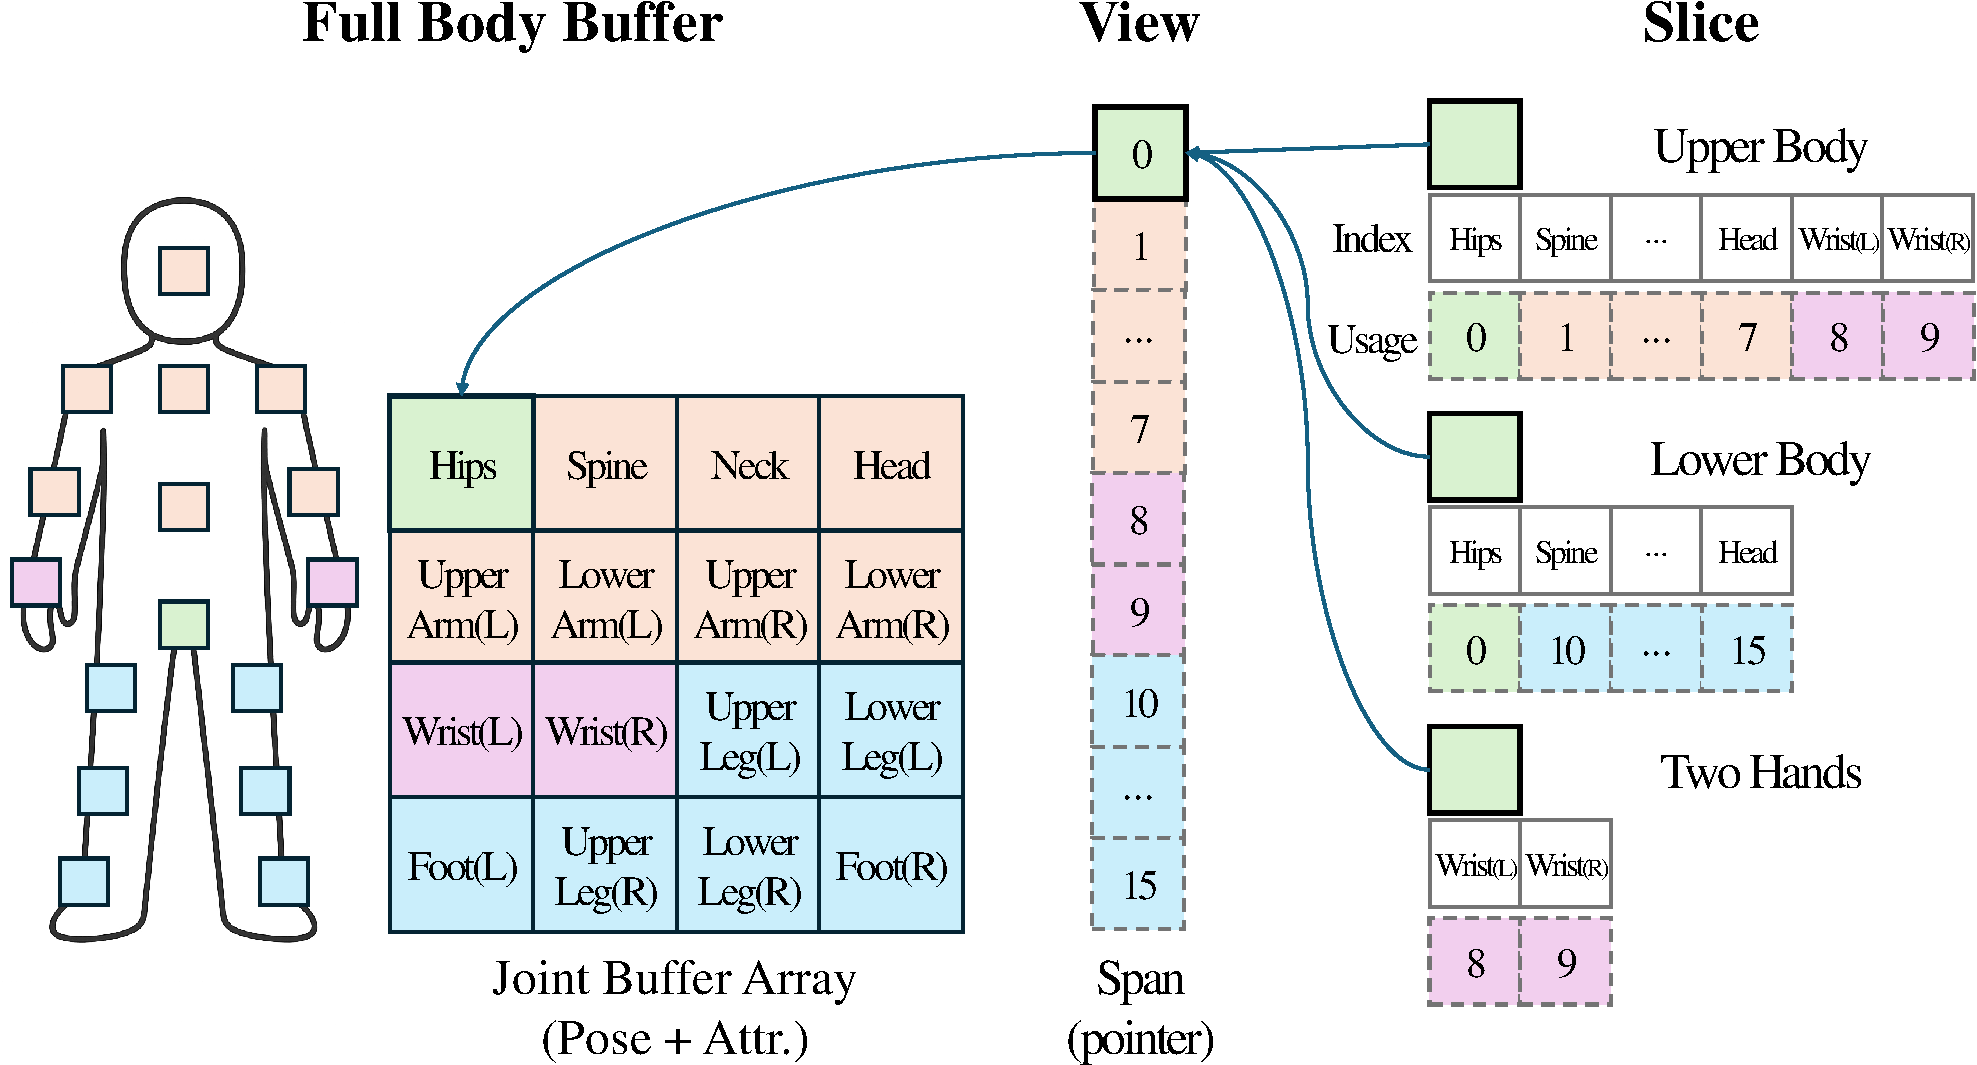
\includegraphics[width=\textwidth]{fig2-kinematicbuffer.pdf}
\caption{Prototype buffer and region-view instantiation of the schema-based motion-data contract. The figure illustrates how a concrete full-body layout is exposed through buffer views for downstream nodes. The slot count shown in the prototype is an implementation example; the conceptual contribution is the schema and validity boundary.}
\label{fig:contract}
\end{figure}

Table~\ref{tab:contract} separates the general contract from the current prototype instantiation. This separation is essential. The prototype's 77-slot layout is useful evidence that the contract can express a full-body avatar pipeline while remaining one schema instantiation.

\begin{table}[t]
\caption{Motion contract concepts. The prototype instantiation is evidence of implementation scope; the conceptual boundary is the schema and validity model.}\label{tab:contract}
\scriptsize
\begin{tabularx}{\textwidth}{P{23mm}YYY}
\toprule
Concept & General definition & Prototype instantiation & Limitation \\
\midrule
Skeleton schema & Defines addressable motion slots and optional parent relations. & Full-body schema with 77 slots covering torso, limbs, head, and articulated hands. & Schema agreement is required between adapters and consumers. \\
Region view & Named subset of slots for partial-body processing. & Views for hands, upper body, lower body, and full body. & Views are implementation-defined rather than discovered from arbitrary rigs. \\
Pose record & Optional components attached to a slot. & Position, rotation, velocity, and scalar angular velocity fields in a per-slot record. & Angular velocity is under-specified for full 3D rotation if represented as a scalar. \\
Validity & Binary component-level availability. & Flags indicate whether position, rotation, velocity, or angular velocity is present. & Continuous confidence is not preserved in the current contract. \\
Buffer view & In-process access to preallocated records. & Kinematic buffer views expose whole-body or region-specific views. & Zero-copy applies only to in-process views, not network transport. \\
Wire format & Serialization follows the same validity contract. & Invalid components can be omitted during serialization. & This paper treats serialization as semantic preservation; compression effects are unevaluated. \\
\bottomrule
\end{tabularx}
\end{table}

Partial tracking is the normal case in XR. A headset and controllers provide only a few rigid poses; a hand tracker may provide fingers but no lower body; a vision model may provide upper-body positions with unreliable rotations; and a full-body SDK may infer unobserved joints internally. UnifiedXRMotion therefore treats absence as first-class data rather than as an error. A downstream node that needs rotations can reject or ignore slots whose rotation flag is absent; a filter that only needs positions can still operate when rotations are missing.


\section{Adapter Boundary}\label{sec:adapters}
Adapters are the boundary where native tracking outputs become contract records. Each adapter initializes or reads a source, converts native joint ordering and coordinate conventions into schema slots, marks component validity, and publishes pose records. The individual SDK calls remain vendor-specific wrapper code. The reusable artifact is the boundary: after publication, downstream filters, estimators, retargeters, replay utilities, and network wrappers depend on slot identity and validity semantics rather than on source-specific records.

\begin{figure}[t]
\centering
\resizebox{\textwidth}{!}{%
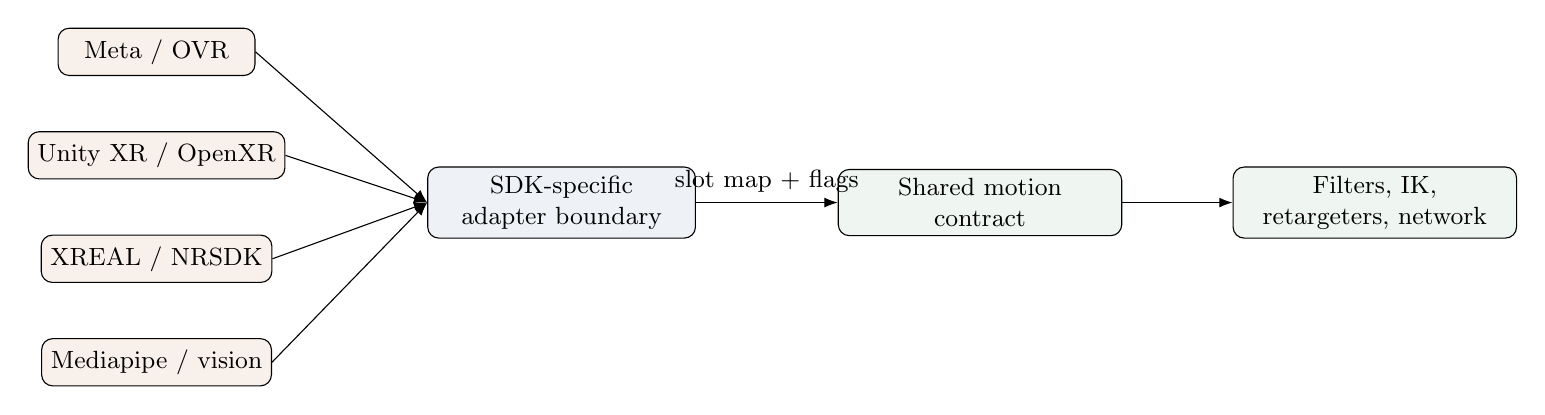
\begin{tikzpicture}[font=\small, node distance=7mm, >=Latex]
  \tikzset{src/.style={draw, rounded corners, align=center, fill=uxorange!10, minimum height=6mm, minimum width=25mm},mid/.style={draw, rounded corners, align=center, fill=uxblue!8, minimum height=8mm, minimum width=34mm},outbox/.style={draw, rounded corners, align=center, fill=uxgreen!8, minimum height=8mm, minimum width=36mm}}
  \node[src] (a) {Meta / OVR};
  \node[src, below=of a] (b) {Unity XR / OpenXR};
  \node[src, below=of b] (c) {XREAL / NRSDK};
  \node[src, below=of c] (d) {Mediapipe / vision};
  \node[mid, right=18mm of b, yshift=-6mm] (adapter) {SDK-specific\\adapter boundary};
  \node[outbox, right=18mm of adapter] (contract) {Shared motion\\contract};
  \node[outbox, right=14mm of contract] (nodes) {Filters, IK,\\retargeters, network};
  \draw[->] (a.east) -- (adapter.west);
  \draw[->] (b.east) -- (adapter.west);
  \draw[->] (c.east) -- (adapter.west);
  \draw[->] (d.east) -- (adapter.west);
  \draw[->] (adapter) -- node[above]{slot map + flags} (contract);
  \draw[->] (contract) -- (nodes);
\end{tikzpicture}%
}
\caption{Adapter boundary. Native tracking sources remain SDK-specific, but each adapter maps observed data into the same schema-based motion contract.}
\label{fig:adapters}
\end{figure}

\begin{table}[t]
\caption{Prototype adapter matrix. The table reports implementation coverage; validation depth differs by source.}\label{tab:adapters}
\scriptsize
\begin{tabularx}{\textwidth}{P{22mm}P{25mm}P{25mm}YY}
\toprule
Adapter/source & Native SDK or source & Motion coverage & Mapping into contract & Validation status and limitation \\
\midrule
Meta body/hand & OVR / OpenXR paths & Body, hands, HMD, controllers & Native bone IDs and device poses are mapped to schema slots. & Implemented and used in prototype traces; remains vendor-specific wrapper code. \\
XREAL hand & NRSDK / XR Hands path & Hands and head-relative context & Hand joints are mapped to hand-region slots with vendor-specific offsets. & Implemented; evidence is limited to adapter functionality rather than avatar-quality assessment. \\
Unity XR & Unity XR / OpenXR input & HMD, controller, hand sources & Generic Unity poses are published into selected slots. & Implemented as adapter evidence for selected OpenXR-style sources. \\
Vive / OpenXR & Vive OpenXR hand tracking & Hand joints & Vendor hand joints are converted to hand-region slots. & Implemented; separate user-study evidence was not collected. \\
Mediapipe & Vision-based landmarks & Hands or upper body & Landmarks are converted into slot positions and binary validity. & Implemented; continuous confidence is quantized away. \\
Android AR / transform / replay / dummy & Mobile AR camera, scene transforms, recorded data, synthetic sources & Application-specific partial motion & Poses are published into selected slots for testing or replay. & Useful for testing and demos; hardware generalization remains outside this evidence. \\
\bottomrule
\end{tabularx}
\end{table}

\begin{table}[t]
\caption{Examples of source-specific coordinate and data-format differences handled at the adapter boundary.}\label{tab:sdk-mapping}
\scriptsize
\begin{tabularx}{\textwidth}{P{20mm}P{22mm}P{27mm}P{31mm}P{23mm}Y}
\toprule
Source / SDK & Native format & Native coordinate convention & Contract mapping & Published region & Valid components / limitation \\
\midrule
Unity OpenXR & 26 $\times$ 6DoF hand joint poses & Left-handed, Z-forward tracking space & Direct slot mapping for hand joints. & Hand slots & Position and rotation valid where provided by Unity XR Hands. \\
Meta OpenXR & 26 $\times$ 6DoF hand joint poses & Right-handed, Z-backward & Z-flip for position and rotation before publication. & Hand slots & Position and rotation valid after conversion; remains SDK-specific wrapper logic. \\
Meta OVR & 24 $\times$ 3DoF local joint rotations plus 6DoF root pose & Right-handed, X-forward local frames & Right-to-left conversion, X-to-Z remapping, and local-to-world reconstruction before slot publication. & Hand slots; body/HMD/controller paths in separate adapters & Rotation is native; positions are reconstructed by forward kinematics. \\
XREAL NRSDK & 23 $\times$ 6DoF joint poses & Left-handed, Y-forward & Y-to-Z axis rotation and hand-region slot mapping. & Hand slots and head-relative context & Position and rotation valid after vendor-specific offsets. \\
XREAL OpenXR & 26 $\times$ 6DoF joint poses & Left-handed, Z-forward & Direct OpenXR-style hand mapping. & Hand slots & Position and rotation valid where the runtime exposes joints. \\
Vive OpenXR & 26 $\times$ 6DoF hand joint poses & Right-handed, Z-backward & Z-flip for position and rotation. & Hand slots & Implemented as selected-source evidence; separate study evidence was not collected. \\
MediaPipe Vision Tasks & 21 world landmarks or 33 body landmarks & Camera-centered world landmarks & Normalize landmarks to tracking frame; publish observed landmarks as slot positions. & Hands or upper body & Position valid; rotations are absent or estimated and should be treated cautiously. \\
\bottomrule
\end{tabularx}
\end{table}

\begin{table}[t]
\caption{Same-consumer, different-source evidence. The goal is to show that source-specific logic is localized at the adapter boundary while downstream consumers reuse contract views.}\label{tab:same-consumer}
\scriptsize
\begin{tabularx}{\textwidth}{P{27mm}P{30mm}P{27mm}P{31mm}Y}
\toprule
Pipeline / source & Adapter-specific code & Shared contract view & Reused downstream consumer & Remaining source-specific concern \\
\midrule
Meta body to avatar & OVR/OpenXR body mapping and device-pose extraction. & Full-body or upper-body schema view. & Full-body retarget node and avatar binding. & Vendor body inference quality and coordinate calibration. \\
XREAL hand to avatar & NRSDK/OpenXR hand conversion and head-relative adjustment. & Two-hands region view. & Two-hands retarget node. & Vendor hand-joint offsets and tracking quality. \\
Unity XR HMD/controllers to estimator & Generic Unity pose handlers for HMD and controllers. & Sparse head/wrist/controller slots. & Upper-body regressor, filter, or replay node. & Which sparse slots are physically observed. \\
MediaPipe position stream to processing nodes & Camera-to-tracking normalization and landmark-to-slot mapping. & Position-valid hand or upper-body view. & Position-only filters, record/replay, and network serialization. & Rotation confidence is not preserved as continuous confidence in the current prototype. \\
Replay / dummy sources to testing & Recorded or synthetic pose publication. & Same schema views as live adapters. & Filters, retargeters, and network wrapper tests. & Fidelity depends on recorded data and schema agreement. \\
\bottomrule
\end{tabularx}
\end{table}

Tables~\ref{tab:adapters}, \ref{tab:sdk-mapping}, and~\ref{tab:same-consumer} show the level at which heterogeneity is localized. Coordinate handedness, joint order, inferred-versus-observed components, and source coverage are handled before publication. After publication, consumers access the same region views and validity masks. This table evidence supports the adapter boundary claim without treating vendor-specific wrapper code as a separate research contribution.


\section{Runtime and Local/Remote Node Placement}\label{sec:runtime}
The runtime uses an event-driven motion-node pipeline over the shared contract. A trigger list identifies root nodes that poll or receive new motion data. When a root node updates, it invokes a sender event; downstream receivers subscribe to that event, read the upstream motion contract through buffer views, write their own output records, and publish another update. The execution model is a Unity-oriented event propagation mechanism rather than a graph-optimization scheduler.

\begin{figure}[t]
\centering
\resizebox{\textwidth}{!}{%
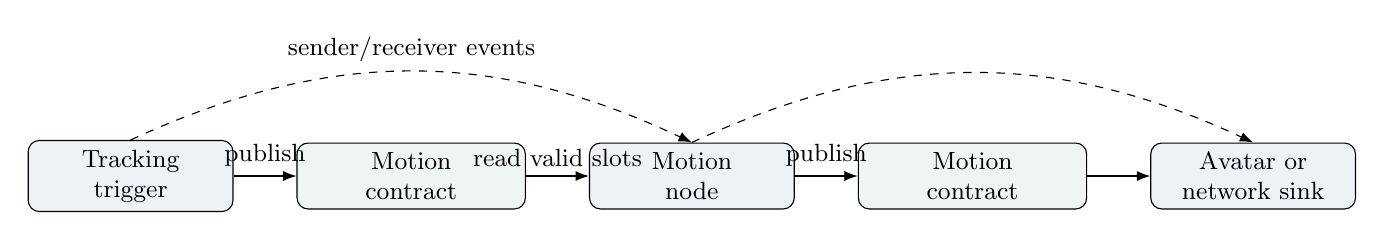
\begin{tikzpicture}[font=\small, node distance=8mm, >=Latex]
  \tikzset{stage/.style={draw, rounded corners, align=center, minimum width=26mm, minimum height=7mm, fill=uxblue!8},contract/.style={draw, rounded corners, align=center, minimum width=29mm, minimum height=7mm, fill=uxgreen!8}}
  \node[stage] (track) {Tracking\\trigger};
  \node[contract, right=of track] (contract) {Motion\\contract};
  \node[stage, right=of contract] (filter) {Motion\\node};
  \node[contract, right=of filter] (contract2) {Motion\\contract};
  \node[stage, right=of contract2] (retarget) {Avatar or\\network sink};
  \draw[->] (track) -- node[above]{publish} (contract);
  \draw[->] (contract) -- node[above]{read valid slots} (filter);
  \draw[->] (filter) -- node[above]{publish} (contract2);
  \draw[->] (contract2) -- (retarget);
  \draw[->, bend left=25, dashed] (track.north) to node[above]{sender/receiver events} (filter.north);
  \draw[->, bend left=25, dashed] (filter.north) to (retarget.north);
\end{tikzpicture}%
}
\caption{Runtime model. UnifiedXRMotion uses trigger-based scheduling and sender/receiver event propagation over a shared motion contract.}
\label{fig:runtime}
\end{figure}

For client-server deployments, UnifiedXRMotion provides a network wrapper around selected motion nodes. The wrapper exposes placement states describing where the producer, node execution, and consumer reside. The claim is structural: a node can be wrapped for different placements without rewriting the node implementation, while behavioral equivalence and performance remain empirical properties of a particular deployment.

\begin{figure}[t]
\centering
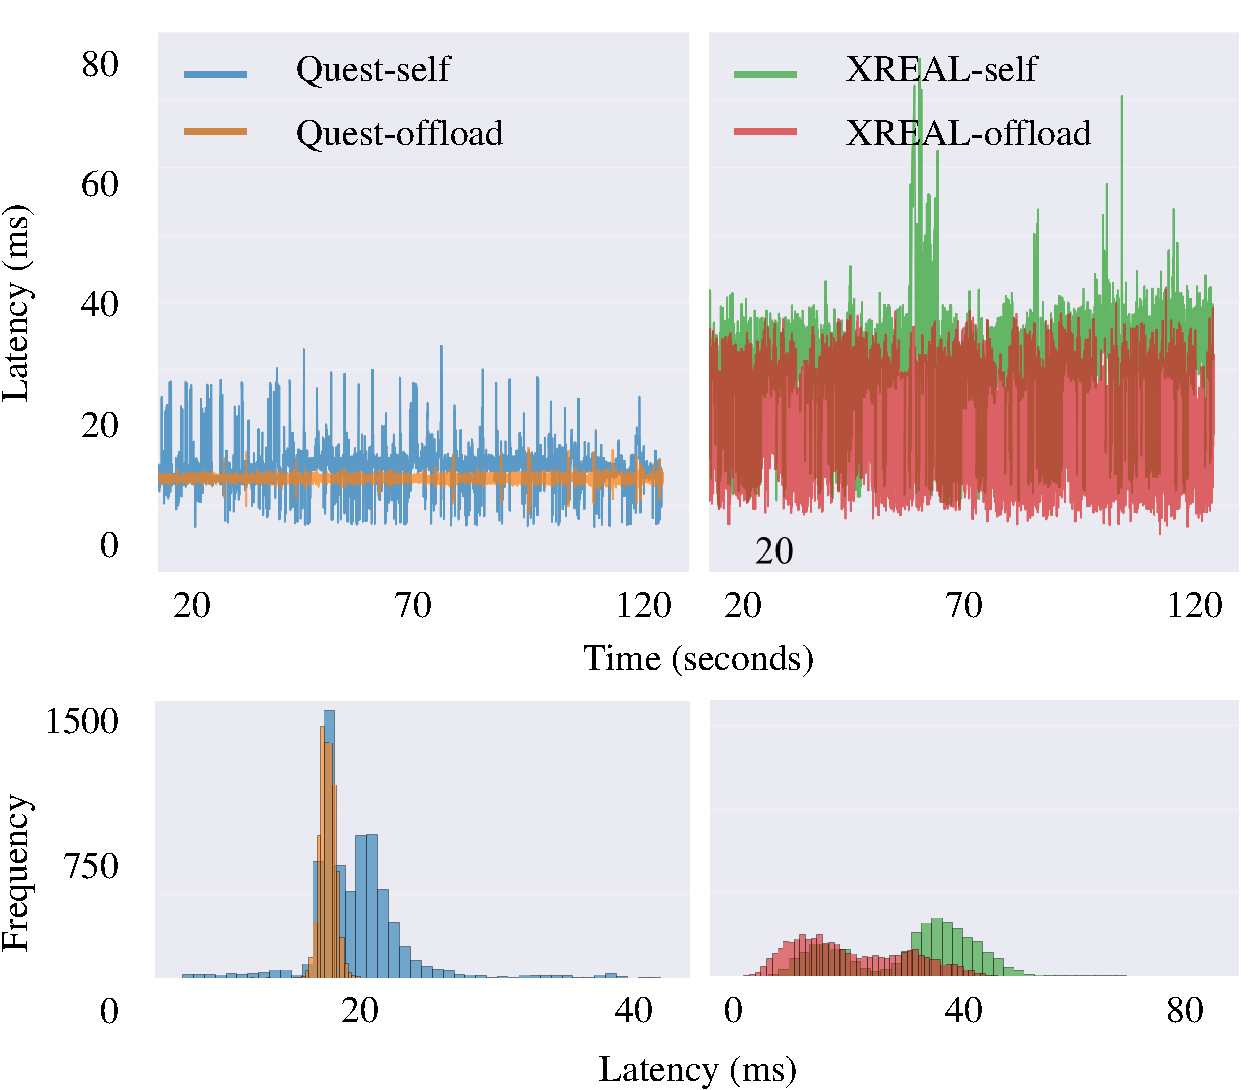
\includegraphics[width=0.92\textwidth]{fig6-offload.pdf}
\caption{Local/remote node-placement abstraction in the prototype. The same class of motion-node pipeline can be configured for local or remote execution contexts through a wrapper.}
\label{fig:placement}
\end{figure}

The timing utility logs application-level motion-pipeline or RPC timing between stamped send and receive events. The metric excludes sensor exposure, SDK internal sampling, Unity render submission, compositor scheduling, and display scan-out. Table~\ref{tab:latency-definition} defines the measurement boundary.

\begin{table}[t]
\caption{Latency metric definition for application-level placement traces.}\label{tab:latency-definition}
\scriptsize
\begin{tabularx}{\textwidth}{P{26mm}YYYP{25mm}}
\toprule
Metric & Included components & Excluded components & Safe interpretation & Unsafe interpretation \\
\midrule
Application-level motion-pipeline latency & Runtime tick/RPC delivery path between stamped motion-buffer send and receive events, plus framework scheduling effects included in that path. & Sensor sampling, native SDK buffering, clock synchronization, rendering, compositor, scan-out, and display timing. & Descriptive timing of the prototype's motion-buffer path under specific local/remote placements. & End-to-end display latency, perceived latency, or proof that offloading improves avatar responsiveness. \\
Frame-time logging utility & Unity frame interval or tick records exported for analysis. & Network transport decomposition and tracker capture time. & Runtime diagnostic signal. & Network latency or user-perceived latency by itself. \\
\bottomrule
\end{tabularx}
\end{table}


\section{Implementation}\label{sec:implementation}
The prototype is implemented as a Unity package. Its core implementation separates four concerns. First, motion slots are stored in preallocated buffers. Region views expose subsets of the schema, allowing a hand-only node, upper-body node, or full-body node to operate on the subset it needs. In-process view access avoids copying the entire pose record for each node. Network transmission necessarily serializes records and is not zero-copy. Second, SDK-specific adapters publish native tracking data into the shared contract. Some adapters are direct wrappers over vendor SDKs; others support synthetic transforms, replay, or vision-based sources. Third, the prototype includes IK, retargeting, codebook, filtering, record, and replay nodes as representative consumers of the contract. Textbook solvers such as FABRIK~\cite{aristidou2011fabrik} and codebook-style control inspired by prior work~\cite{starke2024categorical} provide algorithmic background for these consumers. Fourth, the implementation includes CSV and histogram export utilities for timing traces, plus record/replay utilities that can support reproducible evaluation.

\subsection{Representative Consumer: Retargeting Through Contract Views}\label{sec:retarget-consumer}
Retargeting is used here as a representative consumer of the contract rather than as a claimed algorithmic contribution. A retargeter subscribes to a schema view, checks component validity, and maps the valid source transforms into an avatar-specific rig. For body skeleton retargeting, let $\mathbf{T}_{j,\mathrm{src}}^0$ and $\mathbf{T}_{j,\mathrm{src}}(t)$ denote the homogeneous transforms of source joint $j$ at the canonical pose and at time $t$, and let $\mathbf{T}_{j,\mathrm{tgt}}^0$ denote the target avatar's canonical transform. A representative relative-transform mapping is
\begin{equation}
    \mathbf{T}_{j,\mathrm{tgt}}(t) = \mathbf{T}_{j,\mathrm{src}}(t)\,\mathbf{A}_j\,\mathbf{T}_{j,\mathrm{tgt}}^0,
\end{equation}
where $\mathbf{A}_j = (\mathbf{T}_{j,\mathrm{src}}^0)^{-1}$ is a conceptual alignment from the source canonical frame. In the implementation, equivalent alignment is applied through transform composition rather than through a stored separate variable.

Hand retargeting illustrates why source-specific frames should be normalized before downstream consumption. XR hand SDKs expose inconsistent local frames, so the adapter/consumer boundary constructs anatomical reference frames from observable hand geometry. Let $\mathbf{R}_i=[\hat{\mathbf{x}}_i,\hat{\mathbf{y}}_i,\hat{\mathbf{z}}_i]$ denote a reference frame for hand segment $i$, with origin, forward, and lateral reference points $\mathbf{p}_{i}^{(o)}$, $\mathbf{p}_{i}^{(f)}$, and $\mathbf{p}_{i}^{(l)}$. A representative construction is
\begin{align}
    \hat{\mathbf{x}}_i &= \frac{\mathbf{p}_{i}^{(l)}-\mathbf{p}_{i}^{(f)}}{\lVert \mathbf{p}_{i}^{(l)}-\mathbf{p}_{i}^{(f)}\rVert}, \\
    \hat{\mathbf{z}}_i &= \frac{\mathbf{p}_{i}^{(f)}-\mathbf{p}_{i}^{(o)}}{\lVert \mathbf{p}_{i}^{(f)}-\mathbf{p}_{i}^{(o)}\rVert}, \\
    \hat{\mathbf{y}}_i &= s\;\frac{\hat{\mathbf{z}}_i \times \hat{\mathbf{x}}_i}{\lVert \hat{\mathbf{z}}_i \times \hat{\mathbf{x}}_i\rVert},
\end{align}
with $s=+1$ for left hands and $s=-1$ for right hands. This example shows how contract consumers can reuse the same hand-region view after adapter normalization.

\begin{figure}[t]
\centering
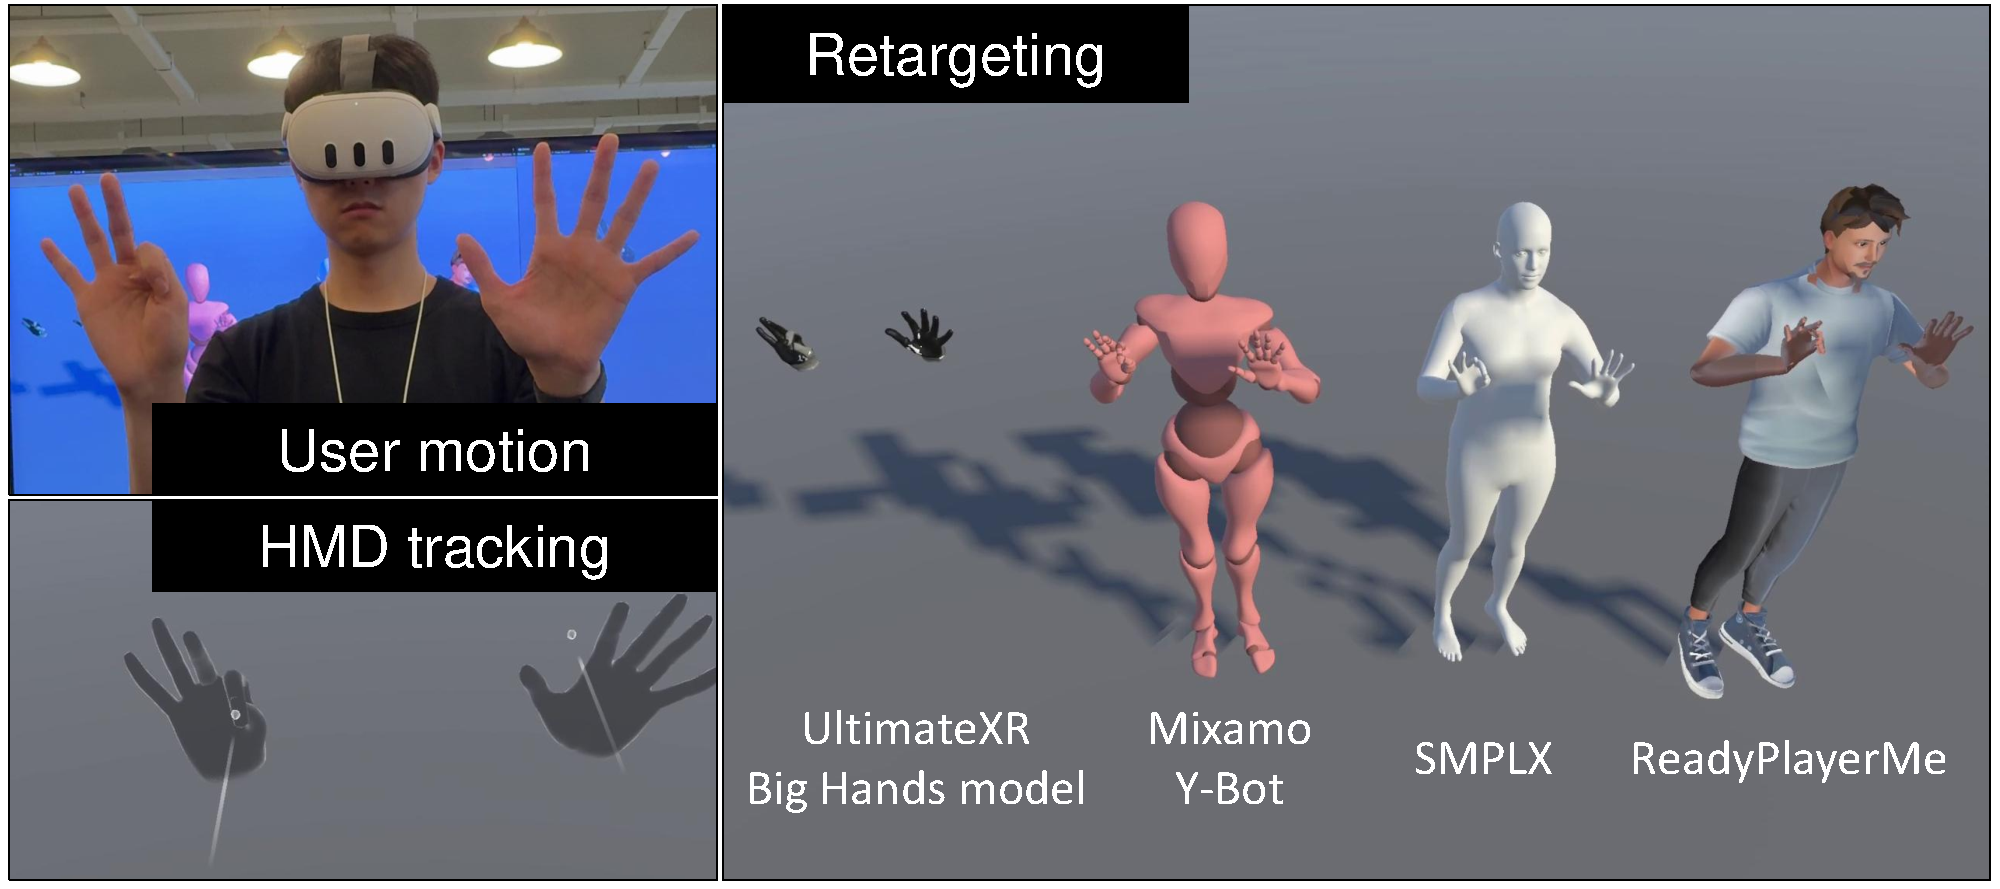
\includegraphics[width=0.92\textwidth]{fig3-retarget.pdf}
\caption{Representative retargeting consumers reading from contract views and writing to heterogeneous avatar rigs. The figure illustrates consumption of the shared motion contract.}
\label{fig:retarget-consumer}
\end{figure}

\begin{table}[t]
\caption{System component classification and evidence scope.}\label{tab:orig-wrapper}
\scriptsize
\begin{tabularx}{\textwidth}{P{25mm}P{27mm}YYY}
\toprule
Component & Classification & Role in this paper & Supported interpretation & Out-of-scope interpretation \\
\midrule
Schema, slot records, validity flags, buffer views & Original framework logic & Motion-data contract & Defines the runtime representation consumed by adapters and nodes. & Universal skeleton standard. \\
Validity-aware serialization & Original logic over networking library & Wire representation & Can omit unavailable components according to flags. & Measured payload reduction without a benchmark. \\
Tracking adapters & SDK-specific wrappers plus mapping logic & Evidence of adapter boundary & Map selected SDK outputs into the shared contract. & New tracking algorithms or universal device support. \\
Event-driven node interfaces & Original runtime logic & Composition model & Supports sender/receiver motion-node pipelines. & Full DAG scheduler or graph optimizer. \\
IK, retargeting, codebook consumers & Textbook, third-party, or application-specific nodes & Example consumers & Demonstrate contract consumption by motion-processing nodes. & Novel IK or retargeting contribution. \\
Network wrapper & Original logic over networking library & Local/remote placement & Provides four structural placement states for wrapped nodes. & Deterministic equivalence or latency improvement without measurement. \\
Timing utilities & Original support code & Descriptive characterization & Export application-level timing traces. & End-to-end display-latency measurement. \\
\bottomrule
\end{tabularx}
\end{table}

\section{Evaluation and Case Study Evidence}\label{sec:evaluation}
The evaluation is designed around the contract-and-boundary systems claim. It asks three questions: whether the schema and validity model are instantiated in a concrete pipeline, whether heterogeneous sources can be localized at adapters while consumers reuse contract views, and how the prototype behaves in one setup task and selected local/remote placement traces. The scope is implementation and application-level evidence for selected pipelines, rather than a complete performance benchmark, avatar-quality study, or device-coverage study.

\subsection{Contract and Adapter Coverage}
Tables~\ref{tab:contract}, \ref{tab:contract-invariants}, \ref{tab:adapters}, \ref{tab:sdk-mapping}, \ref{tab:same-consumer}, and~\ref{tab:orig-wrapper} summarize the implementation evidence for the motion contract, adapter boundary, and original-vs-wrapper separation. The important result is the separation of concerns: device-specific logic is localized in adapters, while downstream nodes operate on the shared contract. This supports the claim that UnifiedXRMotion implements a concrete schema-based contract and demonstrates it with selected sources.

\subsection{Authoring Case Study: Setup Burden}\label{sec:userstudy}
We conducted a within-subjects Unity setup task comparing a UnifiedXRMotion workflow against a vendor SDK workflow. Participants configured the same scene-level goal in both conditions: making custom OpenXR hand prefabs follow simulated hand motion and making the same Y Bot avatar follow simulated full-body motion. Both conditions used the Meta XR Simulator for verification, including random full-body motion and hand motion or pinch gestures. The study used Unity 6000.0.33f1 and Meta Core, Movement SDK, and XR Simulator version 78.0.0.

To avoid conflating pipeline assembly with mesh-specific hand-axis calibration, custom hand retargeting and axis alignment were completed before each session. This made the comparison conservative with respect to UnifiedXRMotion's automatic hand-retargeting support, but it also means the study does not measure the full cost of integrating a previously unseen hand mesh. Participants were instructed to prioritize correctness and completion rather than speed. We therefore interpret completion time as a coarse measure of procedural setup burden, not as a pure speed-optimization measure.

\begin{figure}[t]
\centering
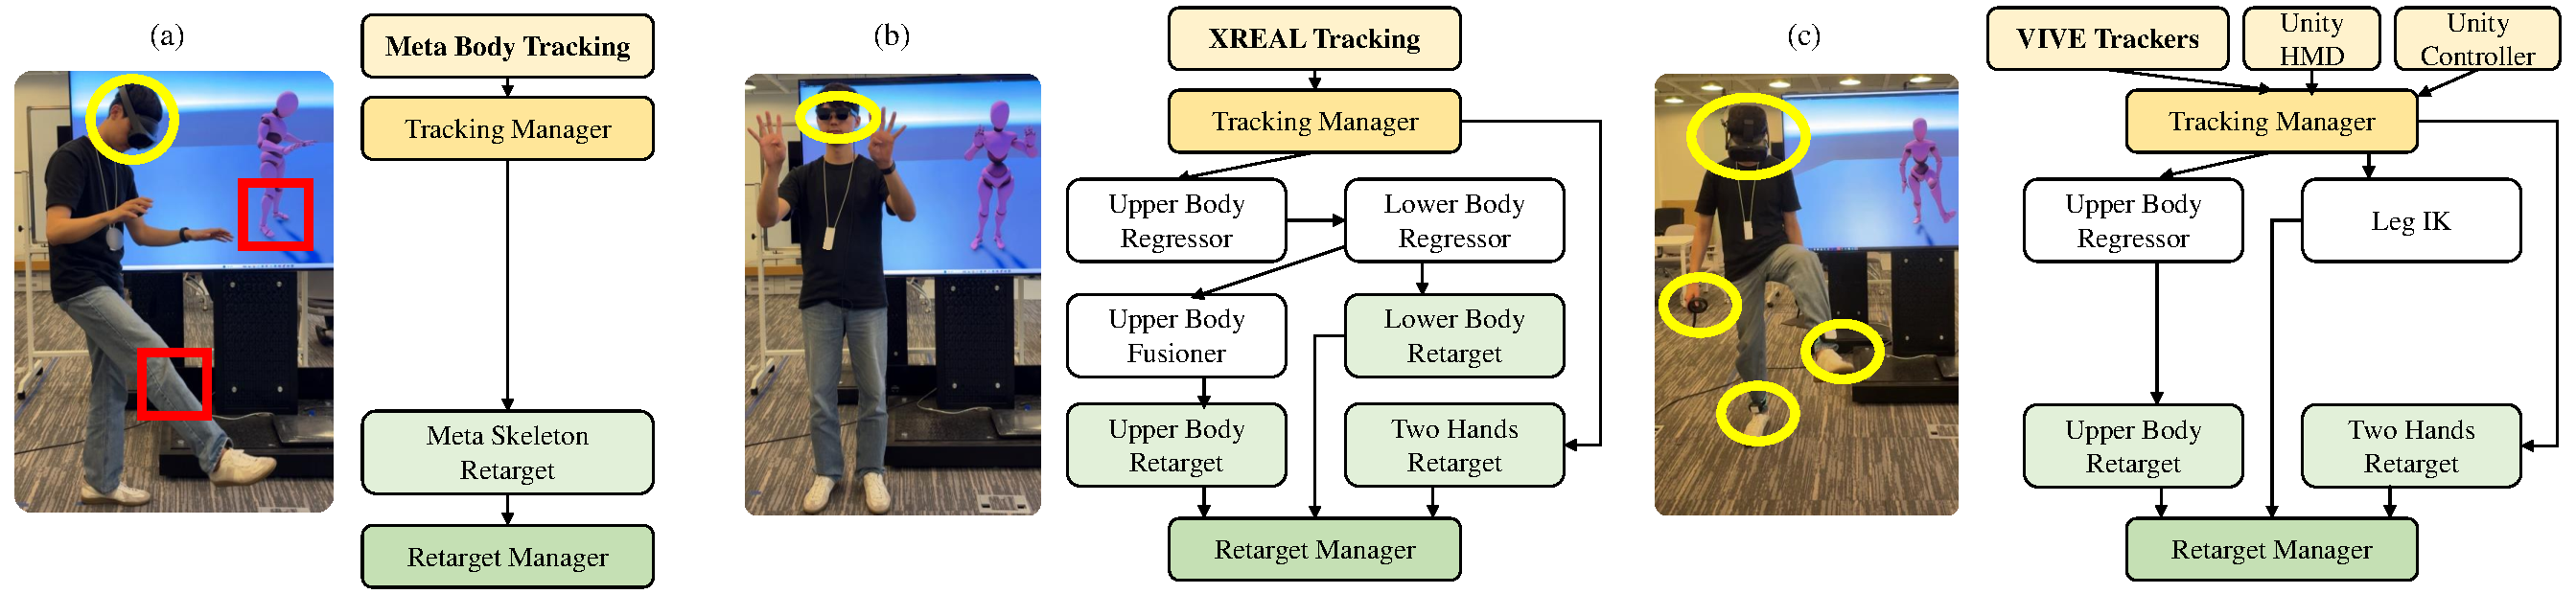
\includegraphics[width=0.92\textwidth]{fig5-configure.pdf}
\caption{Representative setup workflow used in the authoring case study. The figure clarifies the procedural configuration burden measured by the study.}
\label{fig:configure-workflow}
\end{figure}

\begin{table}[H]
\caption{Task-equivalence summary for the authoring case study. SDK A corresponds to UnifiedXRMotion; SDK B corresponds to the vendor SDK workflow.}\label{tab:task-equivalence}
\scriptsize
\begin{tabularx}{\textwidth}{P{23mm}YYP{28mm}}
\toprule
Aspect & UnifiedXRMotion condition & Vendor SDK condition & Interpretation / limitation \\
\midrule
Scene assets & Task scene with Y Bot, Hands, and OpenXR custom hand prefabs. & Matched task scene with the same semantic assets. & Same scene-level goal, not identical procedures. \\
Full-body goal & Add Motion Avatar, MotionSystem, Meta body tracking, and full-body retarget node. & Configure camera rig, body tracking support, and Movement SDK retargeter. & Measures setup burden for one prepared full-body task. \\
Hand goal & Add Motion Avatar, MotionSystem, Meta hand tracking, and two-hands retarget node. & Configure interaction prefabs, synthetic hands, custom skeleton visuals, and data modifiers. & Vendor task has more visible prefab wiring; that is part of the compared workflow. \\
Verification & Meta XR Simulator random body motion and hand/pinch checks. & Same simulator-based behavioral check. & Verifies scene behavior; avatar-motion quality is outside the study scope. \\
Hand-axis alignment & Pre-completed before the session. & Pre-completed before the session. & Avoids a confound but excludes full new-mesh integration cost. \\
Completion criterion & Scene behavior matches reference clips. & Scene behavior matches reference clips. & Completion depends on procedural correctness. \\
\bottomrule
\end{tabularx}
\end{table}

\begin{table}[H]
\caption{Within-subjects setup-burden results ($N=19$). Values are mean $\pm$ standard deviation. NASA--TLX is the 0--100 workload score after reversing the performance subscale so that higher values consistently indicate higher workload. Completion time is interpreted as procedural setup burden because participants prioritized correctness and completion rather than speed.}\label{tab:user-results}
\scriptsize
\centering
\begin{tabularx}{\textwidth}{P{27mm}rrr}
\toprule
Statistic & Completion time (s) & NASA--TLX & SUS \\
\midrule
UnifiedXRMotion ($M\!\pm\!SD$) & $564.03\!\pm\!176.58$ & $30.53\!\pm\!17.55$ & $73.42\!\pm\!17.08$ \\
Vendor SDK ($M\!\pm\!SD$) & $972.89\!\pm\!243.36$ & $49.74\!\pm\!18.29$ & $34.47\!\pm\!13.91$ \\
95\% CI (UXM $-$ SDK) & $[-493.25,\,-324.48]$ & $[-24.87,\,-13.55]$ & $[28.69,\,49.21]$ \\
$t(df)$ & $-10.18\,(18)$ & $-7.13\,(18)$ & $7.98\,(18)$ \\
$p$ & $<.0001$ & $<.0001$ & $<.0001$ \\
Hedges' $g_{\mathrm{av}}$ & $-1.84$ & $-1.03$ & $+2.39$ \\
\bottomrule
\multicolumn{4}{@{}p{\textwidth}@{}}{CIs, $t$, $p$, and effect sizes are computed on paired differences. These statistics are carried over from the existing study analysis; no new user-study measurements were added.}
\end{tabularx}
\end{table}

Table~\ref{tab:user-results} suggests that the UnifiedXRMotion workflow reduced procedural setup burden and improved subjective usability for the tested task. The result is limited to the tested XR setup task: participants did not author new adapters, did not integrate a previously unseen hand mesh, and did not evaluate long-term maintainability. The completion-time result also showed a sequence-sensitive pattern across the counterbalanced orders (mean difference $-307.6$~s for AB and $-521.4$~s for BA; Welch test $t(16.94)=3.32$, $p=.0040$), so the time difference is best interpreted as evidence of procedural burden in this task rather than as a stable developer-speed estimate. Sequence sensitivity was not observed for NASA--TLX ($t(16.10)=-0.31$, $p=.763$) or SUS ($t(16.99)=1.53$, $p=.145$).

\subsection{Case Study: Local and Remote Motion-Node Placement}\label{sec:placement-case}
UnifiedXRMotion allows selected motion nodes to be configured under local or remote placement. We use the traces in this subsection to illustrate this capability: a motion-buffer path can be placed differently and inspected with the prototype's logging utilities. The measurements characterize behavior exposed by the node-placement abstraction in the tested prototype.

The metric is application-level motion-pipeline latency. It includes runtime and network-wrapper timing captured by the prototype, but excludes tracker capture, SDK internal sampling, compositor scheduling, display scan-out, and perceived visual response. Table~\ref{tab:latency-summary} reports the available traces.

\begin{figure}[t]
\centering
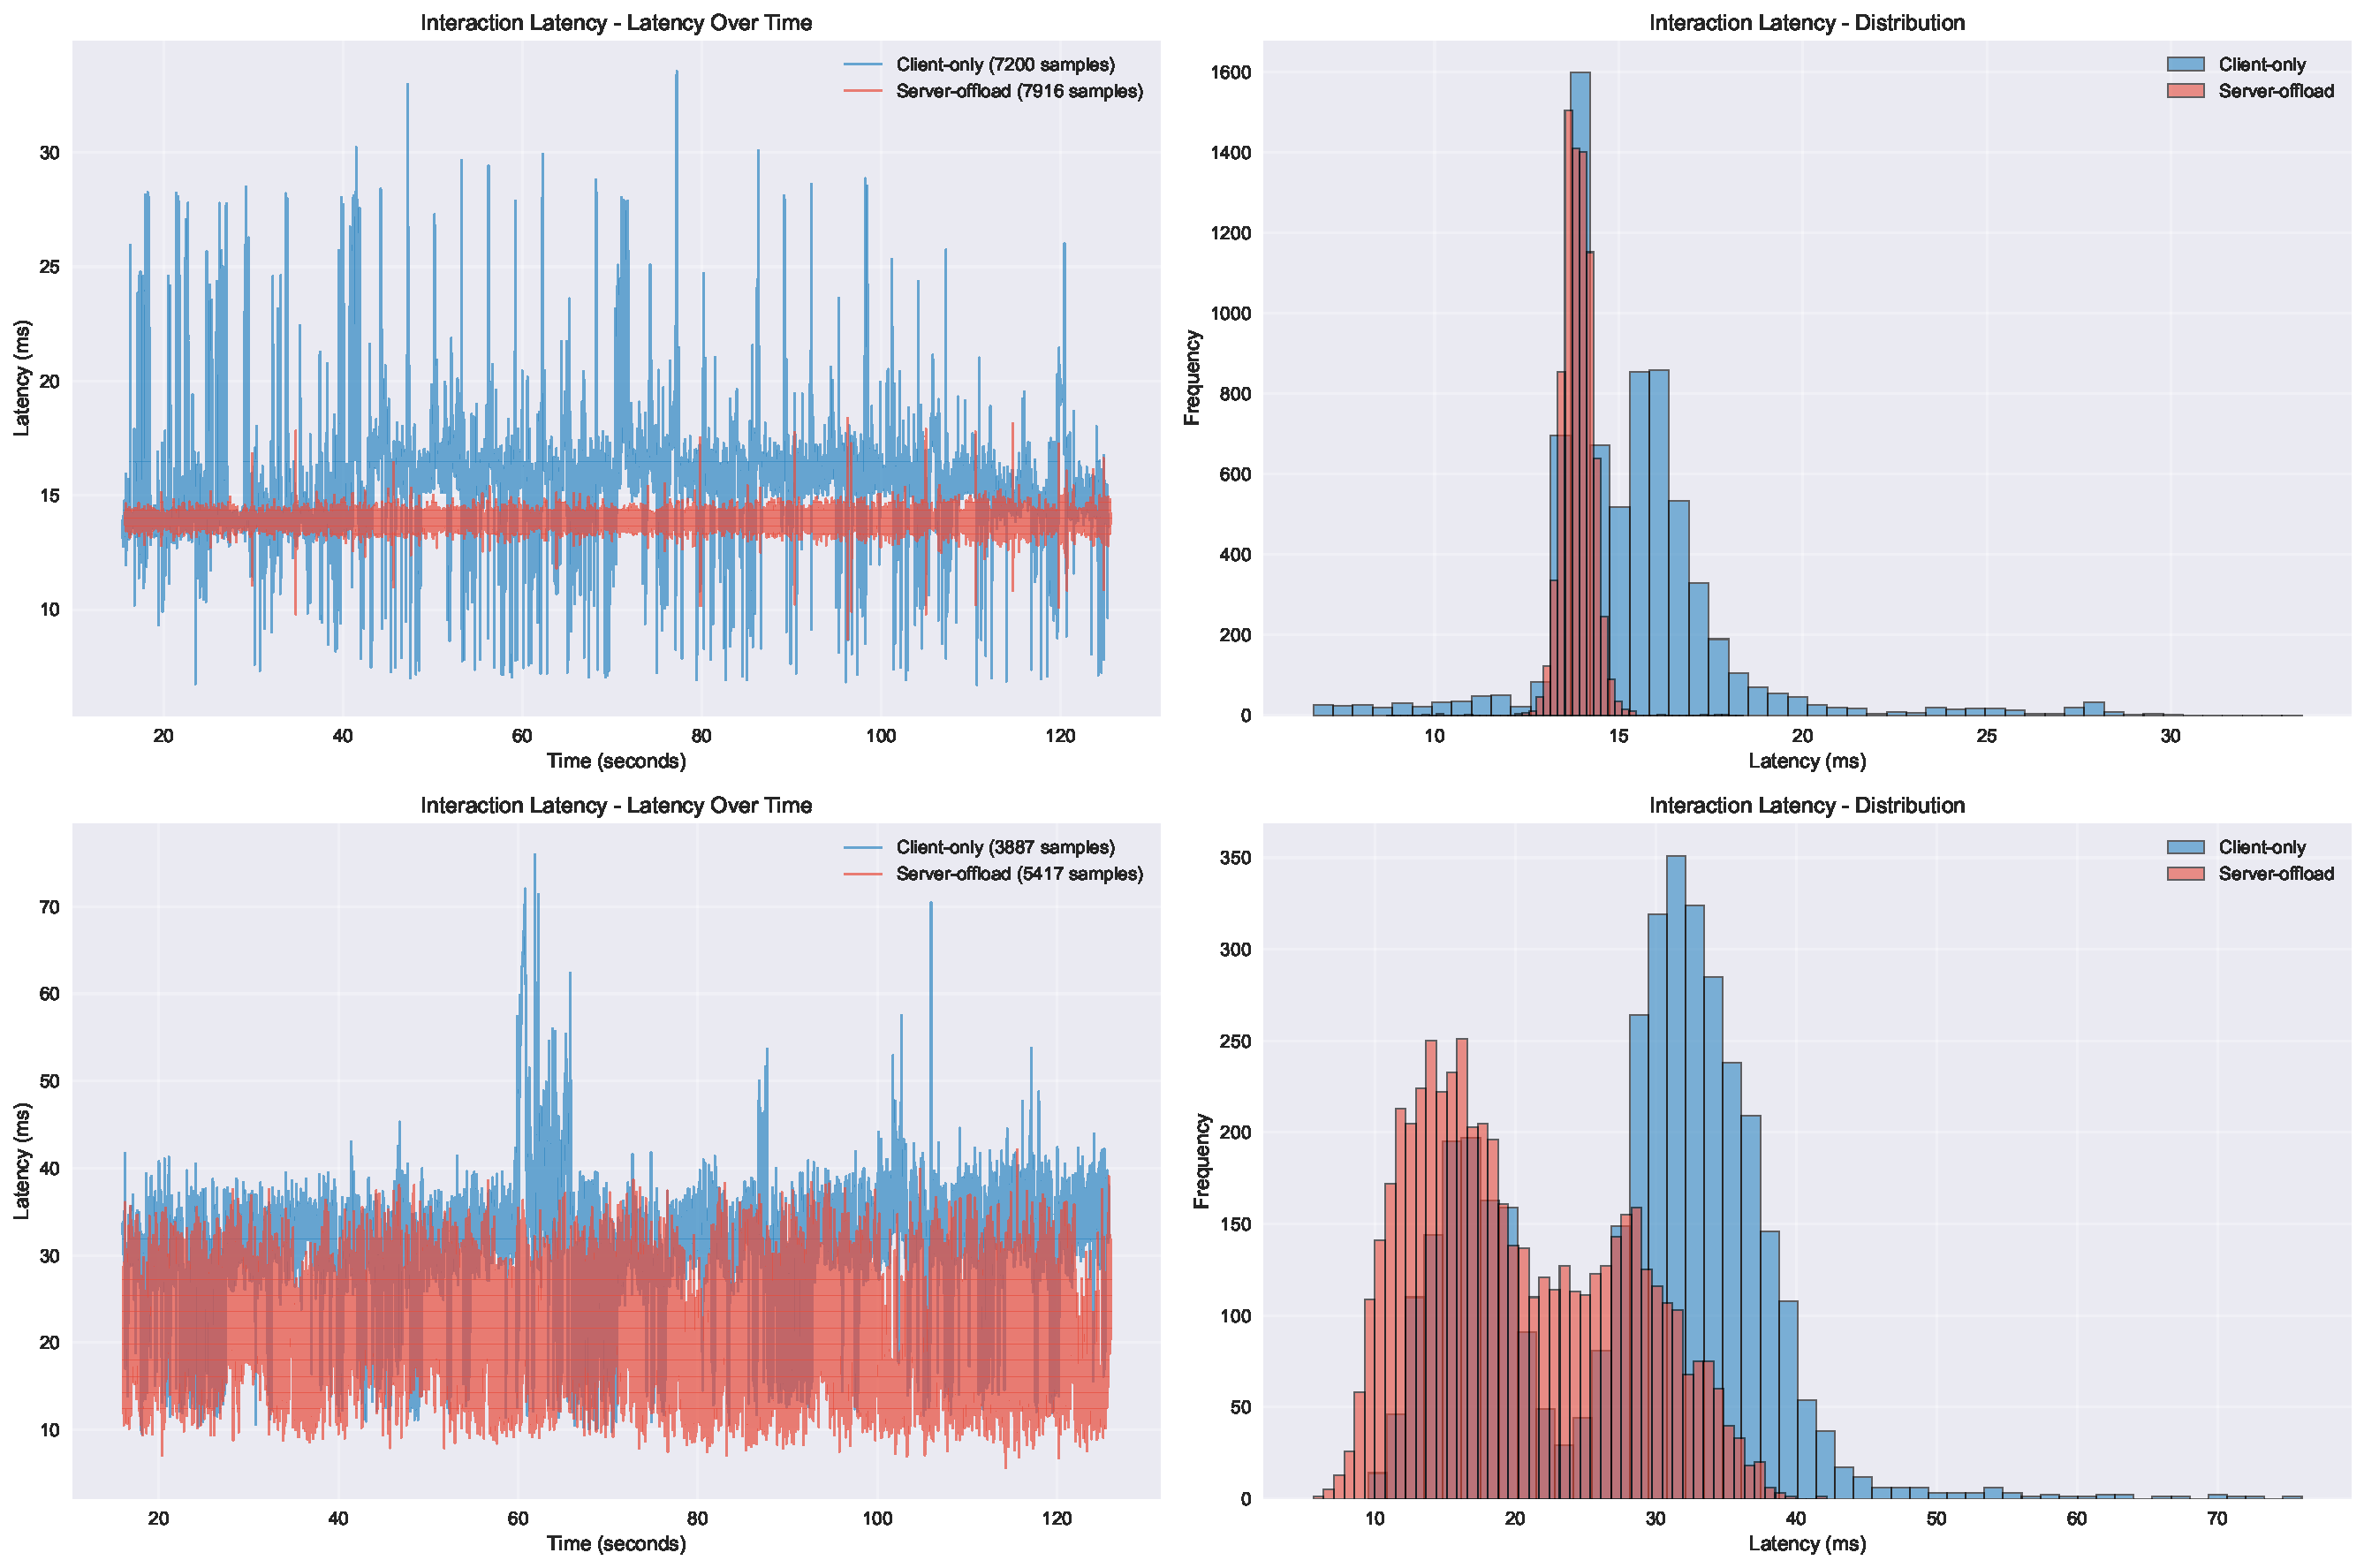
\includegraphics[width=0.96\textwidth]{tick_comparison_analysis.pdf}
\caption{Application-level motion-pipeline latency traces under local and remote node-placement configurations. The plots characterize runtime behavior exposed by the placement abstraction and exclude tracker capture, SDK-internal sampling, compositor scheduling, display scan-out, and perceived visual response.}
\label{fig:latency-placement}
\end{figure}

\begin{table}[H]
\caption{Application-level motion-pipeline latency under local and remote node-placement configurations. Each condition is a trace, not an independent repeated-run distribution.}\label{tab:latency-summary}
\scriptsize
\centering
\begin{tabular}{llrrrrr}
\toprule
Device & Placement & $n$ & Mean & p50 & p95 & p99 \\
\midrule
Meta Quest 3 & Local path & 7859 & 15.27 & 14.86 & 18.98 & 26.96 \\
Meta Quest 3 & Remote path & 8627 & 13.91 & 13.88 & 14.52 & 14.91 \\
XREAL X4000 & Local path & 4190 & 28.64 & 30.46 & 40.21 & 50.90 \\
XREAL X4000 & Remote path & 5913 & 20.30 & 18.53 & 33.34 & 36.29 \\
\bottomrule
\end{tabular}
\end{table}

These traces support a structural interpretation. In the tested prototype, changing placement changes observed application-level timing distributions, so placement is a visible runtime parameter. The traces are insufficient to attribute the cause of each distributional difference or to compare against vendor-native implementations, because the current instrumentation does not isolate serialization time, network transport, SDK buffering, scheduler effects, device temperature, or native tracker buffering.



\section{Discussion}\label{sec:discussion}
\paragraph{Why a motion contract is the research object.} In avatar-motion pipelines, the hard engineering problem is not only acquiring tracking data; it is keeping track of what a source actually observed, representing that partial data consistently, and making downstream nodes robust to missing components. UnifiedXRMotion addresses that problem through schema-defined slots, component-level validity, adapter-localized coordinate conversion, and reusable region views.

\paragraph{What the abstraction enables.} The contract lets adapters, filters, retargeters, and network serializers share a common representation. It also makes missing data explicit. This is valuable for XR because different trackers expose different body regions and component reliability. A hand source, a sparse controller source, a replay stream, and a vision source can all publish partial motion into the same runtime representation, provided that they agree on the schema.

\paragraph{Open design gaps.} The current prototype lacks full timestamp propagation, explicit coordinate-frame metadata in every record, continuous confidence, and schema-version negotiation. These omissions matter. Without timestamps, latency and synchronization claims are limited. Without coordinate-frame metadata, frame conversions remain adapter-specific and easy to misconfigure. Without continuous confidence, vision trackers lose information when confidence is collapsed into binary validity. Without schema versioning, external tools cannot safely exchange saved motion streams across versions.

\paragraph{Local/remote placement remains structural.} The network wrapper is a useful systems abstraction, but structural reuse is not the same as equivalence. A wrapped node may receive data at different times, serialize different subsets, or run under different scheduling conditions. A future version should run the same recorded motion stream through local and remote placements and report per-slot output differences.

\section{Limitations}\label{sec:limitations}
The main limitation is that UnifiedXRMotion is evaluated as an implemented contract boundary, not as a standardized interchange format or an end-to-end performance system. The reported timing traces exclude sensor sampling, SDK internal processing, compositor scheduling, rendering, and display scan-out. Device coverage is also limited to selected adapters; each new tracker still requires a schema mapping, coordinate conversion, and validation. The current 77-slot schema is one prototype instantiation, and arbitrary avatar rigs require schema agreement plus retargeting between the runtime representation and the avatar-specific skeleton. The included tracking, IK, and retargeting components are representative consumers rather than algorithmic contributions.

The authoring case study also has limits. Hand-axis alignment and mesh-specific retargeting were pre-completed before sessions, so the study isolates pipeline assembly rather than full new-avatar integration. Participants were instructed to prioritize correctness and task completion, so completion time should be interpreted as procedural setup burden, not pure speed. The study does not measure adapter-authoring effort or long-term maintainability. The evaluation also lacks a bytes-per-frame wire-format benchmark, a serialization round-trip test, a deterministic local/remote equivalence check, and a vendor-native runtime latency baseline. These remain the strongest next validation targets.

\section{Conclusion}
\label{sec:conclusion}
UnifiedXRMotion reframes heterogeneous XR avatar-motion integration as a runtime contract problem. It defines a schema-based validity-aware representation in which producers publish partial motion into addressable slots and downstream nodes consume explicitly valid components through shared views. The Unity prototype demonstrates the contract with selected SDK and vision adapters, event-driven motion nodes, representative retargeting and IK consumers, replay utilities, and a local/remote node-placement wrapper. The evidence supports a scoped EuroXR systems contribution: a concrete contract and adapter boundary for composing heterogeneous XR avatar-motion pipelines, with supporting evidence from implementation coverage, a setup-burden case study, and application-level placement traces.

\bibliographystyle{splncs04}
\bibliography{bib/references}
\end{document}
